\documentclass{article}
\usepackage{amsthm,graphicx}

\newtheorem{lem}{Lemma}
\newtheorem{thm}{Theorem}

\begin{document}
A \emph{guillotine subdivision} $S$ is obtained by inserting a sequence 
$s_1,\ldots,s_n$ of line segments.  Each inserted segment $s_i$ splits a face of
the current subdivision $S_{i-1}$ into two new faces yielding a new subdivision $S_i$.

\begin{lem}\label{lem:chop}
Let $F$ be a face in a guillotine subdivision $S$.  If there are
1-transmitters on every face that shares an edge with $F$ then these
1-transmitters see all of $F$.
\end{lem}

\begin{proof}
Consider the segment $s_i$ whose insertion created the face $F$.
Before the insertion of $s_i$, the subdivision $S_{i-1}$ contained
a convex face that was split by $s_i$ into two faces $F$ and $F'$
(Figure~\ref{fig:chop}.a).  No further segments were inserted into
$F$, but $F'$ may have been further subdivided, so that there are now
several faces $F'_1,\ldots,F'_k$, with $F'_j\subseteq F'$ and $F'_j$ incident on $s$ for all $j\in\{1,\ldots,k\}$
(Figure~\ref{fig:chop}.b).

\begin{figure}
  \begin{center}
    \begin{tabular}{ccc}
      
\includegraphics{chop-a} &   
      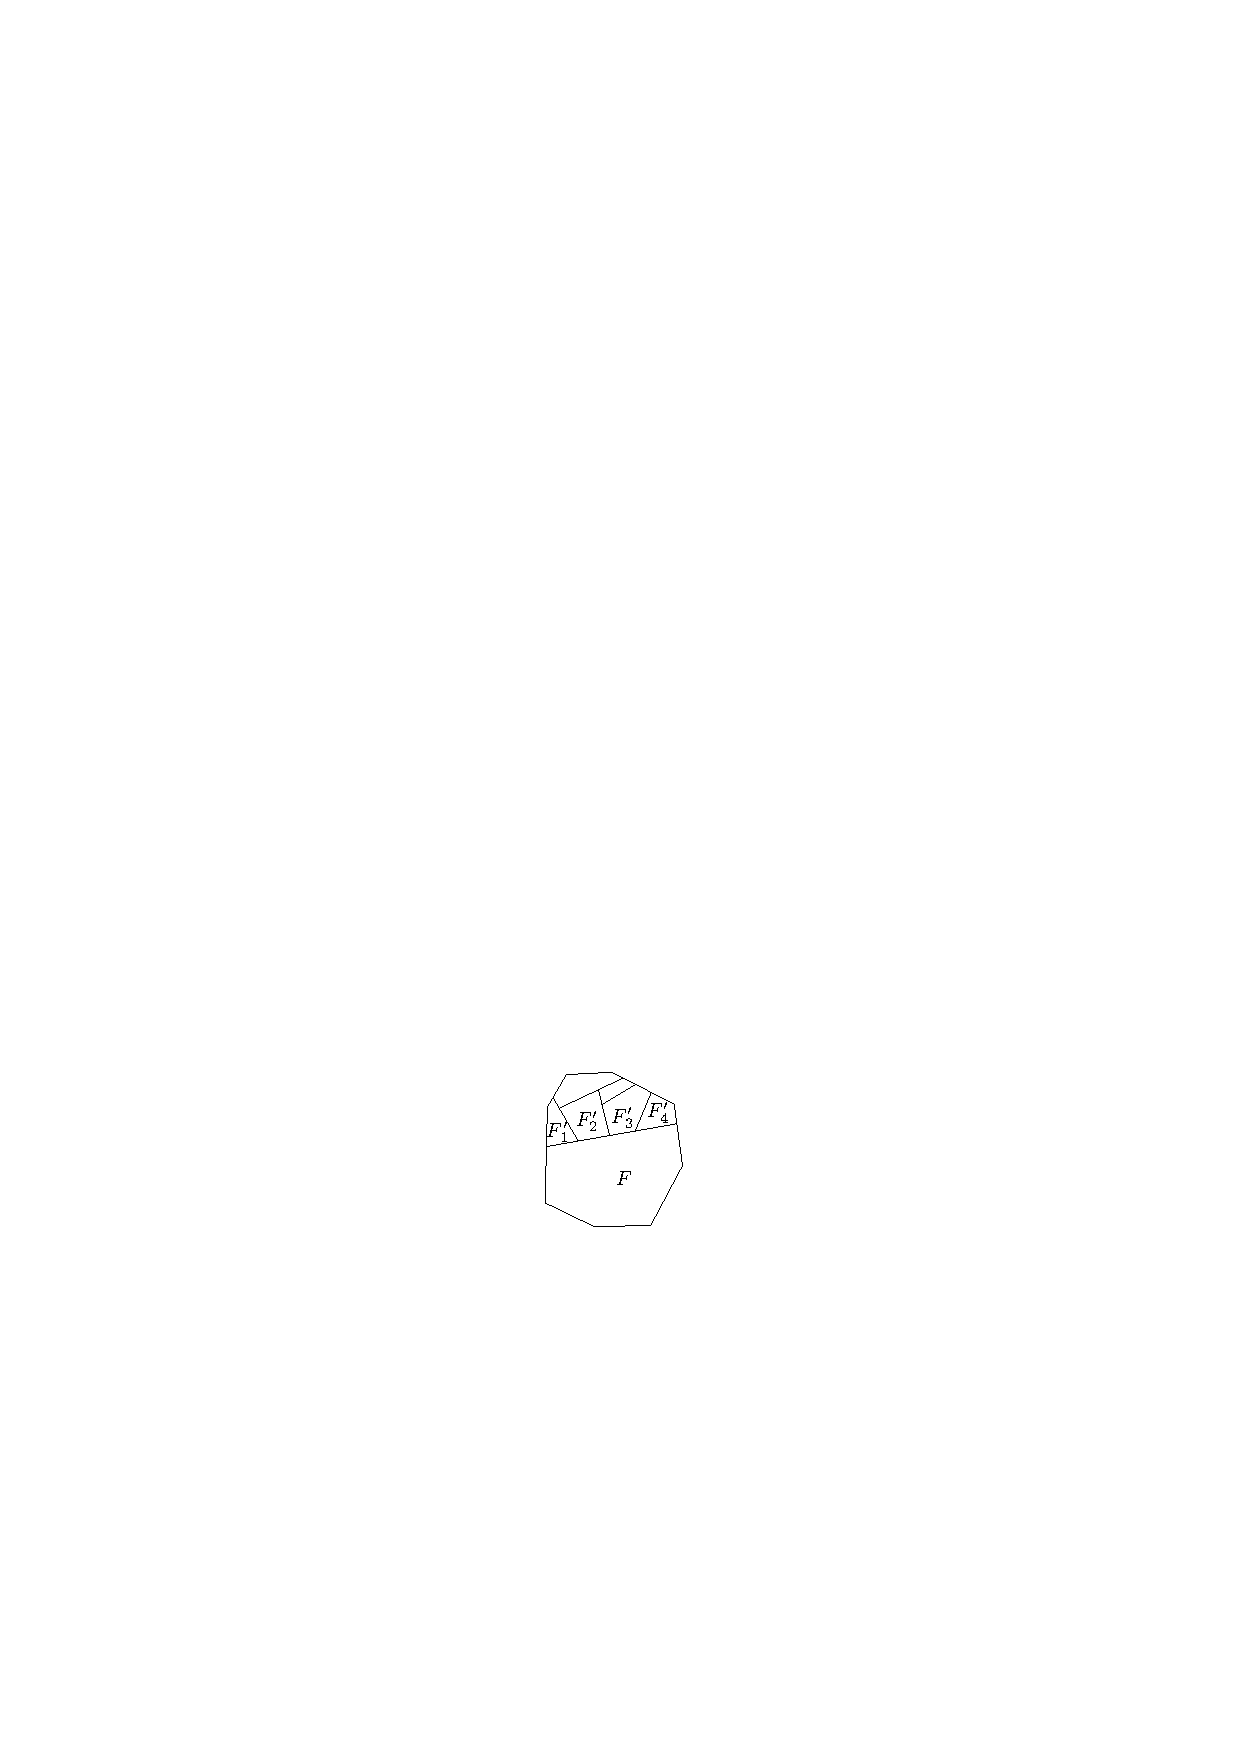
\includegraphics{chop-b} &   
      
\includegraphics{chop-c}  \\  
      (a) & (b) & (c) \\[1ex]
      & 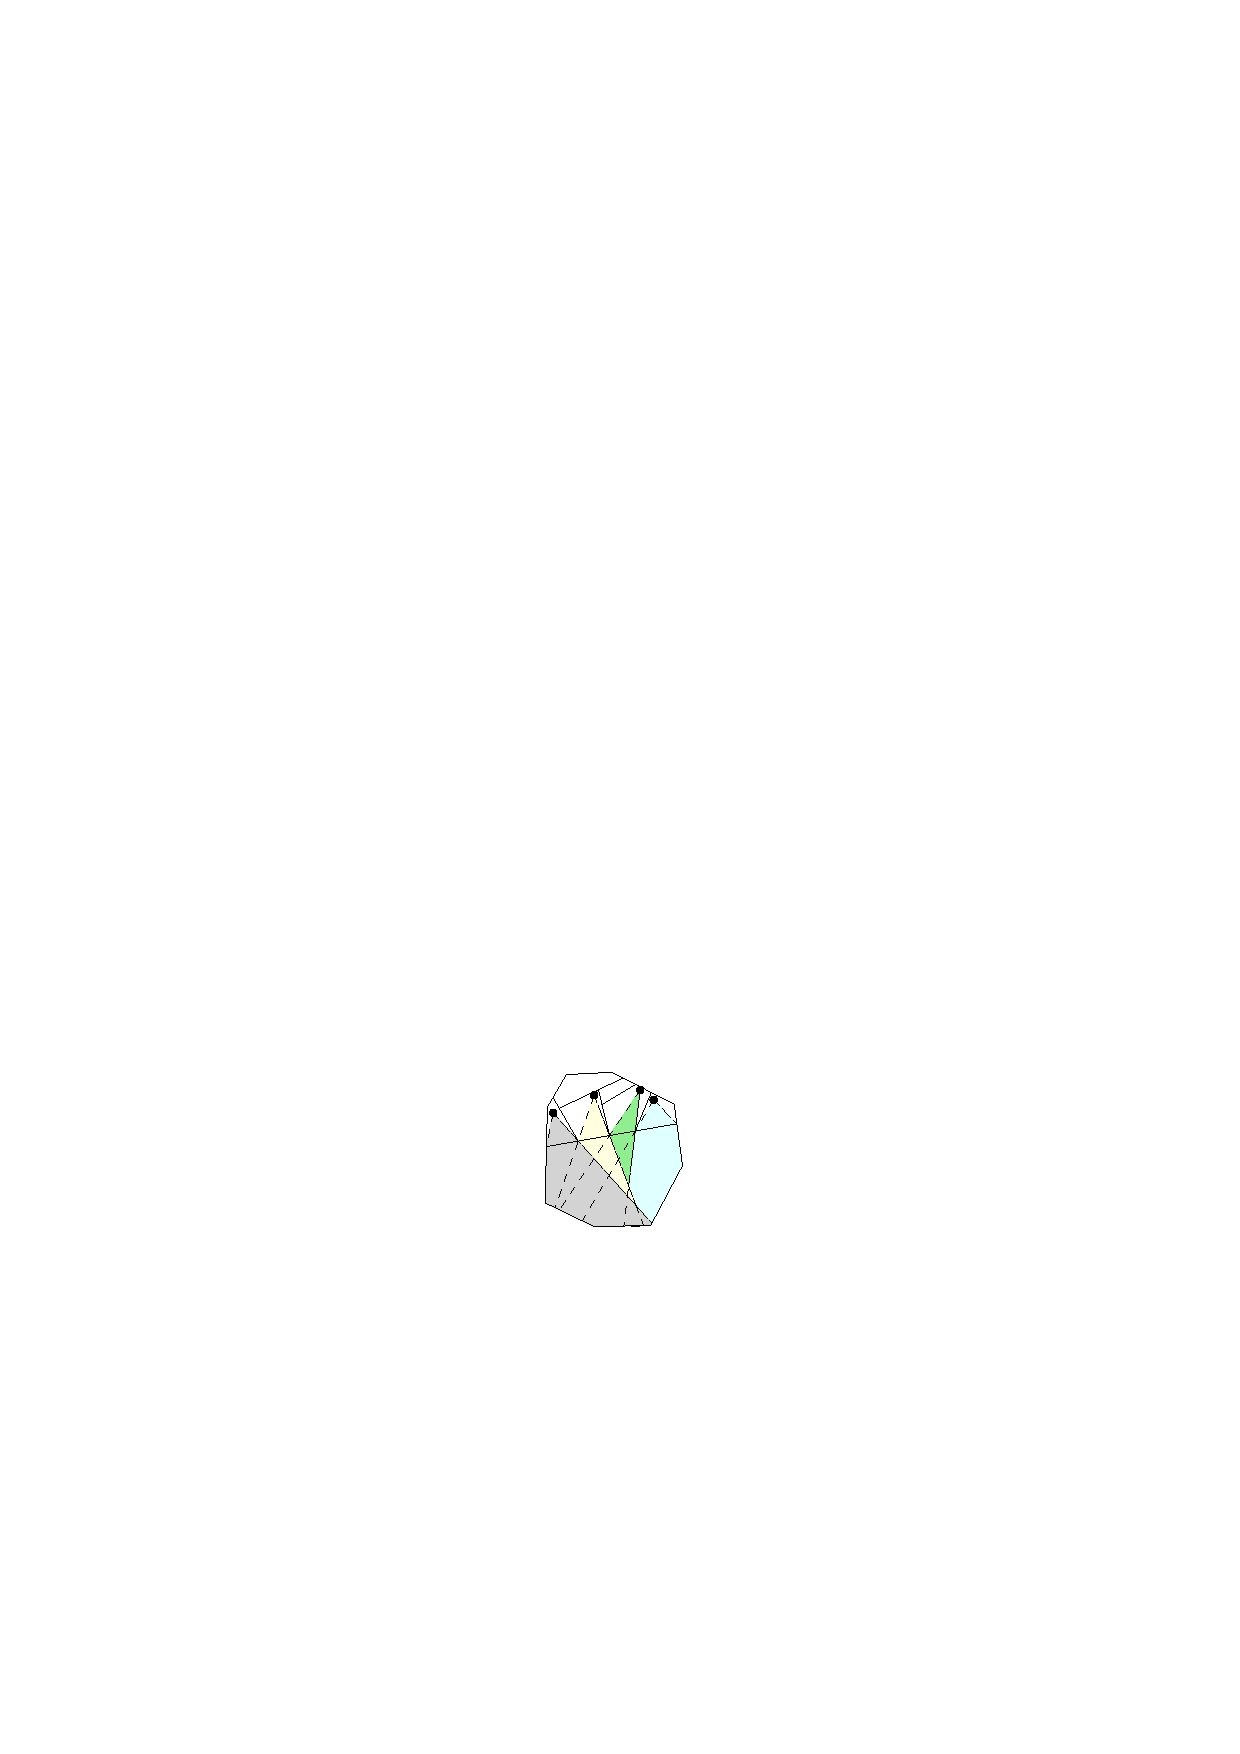
\includegraphics{chop-d} &  \\  
      & (d) &  \\  
    \end{tabular}
  \end{center}
  \caption{The proof of Lemma~\ref{lem:chop}.}
  \label{fig:chop}
\end{figure}

We claim that the 1-transmitters in $F_1',\ldots,F_k'$ guard the interior
of $F$.  To see this, imagine removing $s_i$ from the subdivision and
instead, constructing a guillotine subdivision $\tilde{S}$ from the sequence
$s_1,\ldots,s_{i-1},s_{i+1},\ldots,s_n$ (Figure~\ref{fig:chop}.c).
In this case, each face $F_j'$ in $S$ becomes a larger face $\tilde F_j'$
in $\tilde{S}$ and together $\bigcup_{j=1}^k \tilde F_j'\supseteq F$.  Finally,
we observe that each 1-transmitter in $S$ in face $F_j'$ guards at least
$\tilde F_j'$, so together, the 1-transmitters in $F_1',\ldots,F_k'$
guard all of $F$ (Figure~\ref{fig:chop}.d).
\end{proof}


\begin{thm}
Any guillotine subdivision can be guarded with at most $(n+1)/2$ 1-transmitters.
\end{thm}

\begin{proof}
Consider the dual graph $T$ of the subdivision. $T$ is a triangulation
with $n+1$ faces.  Let $M$ be any maximal matching in $T$.  Consider the
unmatched vertices of $T$.  Each such vertex is adjacent only to matched
vertices (otherwise $M$ would not be maximal).  Let $G$ be the set of
1-transmitters obtained by placing a single 1-transmitter on the primal
edge associated with each edge $e\in M$.  Then $|G|=|M|\le (n+1)/2$.
For every face $F$ of $S$, $F$ either contains a 1-transmitter in $G$,
or all faces that share an edge with $F$ contain a 1-transmitter in $G$.
In the former case, $F$ is obviously guarded. In the latter case,
Lemma~\ref{lem:chop} ensures that $F$ is guarded.  Therefore, $G$ is a set of 1-transmitters that guards all faces of $F$ and has size at most $(n+1)/2$.
%
%
%Therefore, if we construct
%a set of 1-transmitters by placing a guard on the dual of each matched
%edge, we get a set of 1-transmitters for which each face either contains
%a 1-transmitter or all adjacent faces contain a 1 transmitter.
%
%
%
%A \emph{Type~A}
%unmatched vertex $u$ is incident on a triangle (face) of $T$, one
%of whose edges $e$ is in the matching $M$ (Figure~\ref{fig:type}.a).
%We call $(e,u)$ a \emph{Type~A pair}. All other unmatched vertices
%are Type~B.  Note that every neighbour of a Type~B unmatched vertex is
%matched (otherwise $M$ would not be maximal).
%
%Therefore, we construct our 1-transmitter set as follows:  We place a
%1-transmitter $t$ on the primal edge $e'$ that is dual to each edge
%$e$ in $M$.  If $e$ is part of one or two Type~A pairs $(e,u)$ then
%we move $t$ to one endpoint of $e'$ so that it guards three faces,
%two on either side of $e'$ and one incident to an endpoint of $e'$
%(Figure~\ref{fig:type}.b).
%
%Lemma~\ref{lem:chop} guarantees that the above set of 1-transmitters
%guards every Type~B face.  It also guards at least half of the Type~A
%faces and all of the faces corresponding to matched vertices.  The number
%of faces left unguarded is therefore at most
%\[ 
%   (n+1-2|M|)/2  \enspace .
%\]
%By adding an additional 1-transmitter in every remaining unguarded Type~A face, we obtain a guard set of size
%\[
% |M| + (n+1-2|M|)/2 = (n+1)/2  \enspace ,
%\]
%as required.
\end{proof}


\end{document}
